\section{Paper B: AEMS for Gatheral DMR}

\begin{frame}{Paper B: Gatheral DMR as a Non-Affine Extension}
  \keymessage{Paper B moves from Heston-type affine structure to Gatheral DMR, where the stochastic long-run variance improves flexibility but makes simulation less direct.}

  \vspace{0.5em}
  \begin{columns}[T,onlytextwidth]
    \begin{column}{0.52\textwidth}
      \[
      \begin{aligned}
      \dd S_t &= rS_t\dd t+\sqrt{v_t}S_t\dd \widetilde W_t^{(1)},\\
      \dd v_t &= \kappa_1(v'_t-v_t)\dd t+\xi_1\sqrt{v_t}\dd \widetilde W_t^{(2)},\\
      \dd v'_t &= \kappa_2(\theta-v'_t)\dd t+\xi_2\sqrt{v'_t}\dd \widetilde W_t^{(3)}.
      \end{aligned}
      \]
    \end{column}
    \begin{column}{0.42\textwidth}
      \begin{block}{Numerical implication}
        The long-run variance \(v'\) has a CIR structure, but the current variance \(v\) mean-reverts to the stochastic level \(v'\). Therefore the two variance equations cannot be simulated in one closed-form exact step as in the Heston case.
      \end{block}
    \end{column}
  \end{columns}
\end{frame}

\begin{frame}{Paper B Method: AEMS and AEMS-SOR}
  \begin{columns}[T,onlytextwidth]
    \begin{column}{0.48\textwidth}
      \begin{block}{AEMS}
        \begin{itemize}
          \item Extend the Paper A AES idea by using exact CIR sampling where possible.
          \item Sample the long-run variance \(v'\) from its CIR distribution.
          \item Update \(v\) with a Milstein-style correction.
          \item Use the correlation structure in the log-price update.
        \end{itemize}
      \end{block}
    \end{column}
    \begin{column}{0.48\textwidth}
      \begin{block}{AEMS-SOR}
        \begin{itemize}
          \item Adds a second-order refinement.
          \item Aims to improve weak convergence.
          \item Its numerical advantage depends on payoff, maturity, and moneyness.
        \end{itemize}
      \end{block}
    \end{column}
  \end{columns}

  \vspace{0.4em}
  \keymessage{AEMS is a mixed scheme: exact sampling is used for \(v'\), while \(v\) and the log price are updated by approximation formulas.}
\end{frame}

\begin{frame}{Paper B Derivation: AEMS Correlation Decomposition}
  \vspace{-0.8em}
  {\fontsize{4.35}{4.75}\selectfont
  \setlength{\abovedisplayskip}{0pt}
  \setlength{\belowdisplayskip}{0pt}
  \setlength{\jot}{0.05em}
  The Gatheral DMR model is first rewritten with a Cholesky decomposition so that the
  correlated Brownian motions are expressed through independent Brownian motions.
  \vspace{-0.25em}
  \begin{columns}[T,onlytextwidth]
    \begin{column}{0.50\textwidth}
      \begin{block}{1. Integral representation}
        \[
        \resizebox{0.98\linewidth}{!}{$
        \begin{aligned}
        X_{t+\dt}&=X_t+\int_t^{t+\dt}\!\left(r-\tfrac12v_u\right)\dd u
        +\rho^*\!\int_t^{t+\dt}\!\sqrt{v_u}\dd W_u^{(1)}\\
        &\quad+\frac{\rho_{12}-\rho_{13}\rho_{23}}{\sqrt{1-\rho_{23}^2}}
        \int_t^{t+\dt}\!\sqrt{v_u}\dd W_u^{(2)}
        +\rho_{13}\!\int_t^{t+\dt}\!\sqrt{v_u}\dd W_u^{(3)},\\
        v_{t+\dt}&=v_t+\kappa_1\int_t^{t+\dt}(v'_u-v_u)\dd u
        +\xi_1\sqrt{1-\rho_{23}^2}\int_t^{t+\dt}\!\sqrt{v_u}\dd W_u^{(2)}\\
        &\quad+\xi_1\rho_{23}\int_t^{t+\dt}\!\sqrt{v_u}\dd W_u^{(3)},\\
        v'_{t+\dt}&=v'_t+\kappa_2\int_t^{t+\dt}(\theta-v'_u)\dd u
        +\xi_2\int_t^{t+\dt}\!\sqrt{v'_u}\dd W_u^{(3)}.
        \end{aligned}
        $}
        \]
      \end{block}
      \vspace{-0.55em}
      \[
        \resizebox{0.62\linewidth}{!}{$
        \rho^*=\sqrt{1-\rho_{13}^2-
        \frac{(\rho_{12}-\rho_{13}\rho_{23})^2}{1-\rho_{23}^2}}.
        $}
      \]
    \end{column}
    \begin{column}{0.48\textwidth}
      \begin{block}{2. Isolate the shared Brownian part of \(v\)}
        \[
        \resizebox{0.98\linewidth}{!}{$
        \begin{aligned}
        v_{t+\dt}&=v_t+\kappa_1\int_t^{t+\dt}(v'_u-v_u)\dd u\\
        &\quad+\xi_1\rho_{23}\left(
        \frac{\sqrt{1-\rho_{23}^2}}{\rho_{23}}
        \int_t^{t+\dt}\sqrt{v_u}\dd W_u^{(2)}
        +\int_t^{t+\dt}\sqrt{v_u}\dd W_u^{(3)}
        \right).
        \end{aligned}
        $}
        \]
      \end{block}
      \vspace{-0.55em}
      \begin{block}{3. AEMS final one-step form}
        \[
        \resizebox{0.98\linewidth}{!}{$
        \begin{aligned}
        X_{t+\dt}&=X_t+\left(r-\tfrac12v_t\right)\dt
        +\rho^*\sqrt{v_t}\Delta W^{(1)}
        +\rho^{**}\sqrt{v_t}\Delta W^{(2)}\\
        &\quad+\rho_{13}
        \left(\frac{v_{t+\dt}-v_t-\kappa_1(v'_t-v_t)\dt}{\xi_1\rho_{23}}\right),\\
        v_{t+\dt}&=v_t+\kappa_1(v'_t-v_t)\dt
        +\xi_1\sqrt{v_t\dt}\,Z_v
        +\tfrac14\xi_1^2\dt\,(Z_v^2-1),\\
        v'_{t+\dt}&=\bar c(t+\dt,t)\cdot\chi^2\!\left(\delta,\bar\kappa(t+\dt,t)\right),
        \end{aligned}
        $}
        \]
        \[
          \resizebox{0.72\linewidth}{!}{$
          \rho^{**}=
          \frac{\rho_{12}-\rho_{13}\rho_{23}}{\sqrt{1-\rho_{23}^2}}
          -\rho_{13}\frac{\sqrt{1-\rho_{23}^2}}{\rho_{23}}.
          $}
        \]
      \end{block}
    \end{column}
  \end{columns}}
\end{frame}

\begin{frame}{Paper B Derivation: AEMS-SOR Second-Order Correction}
  \vspace{-0.6em}
  {\fontsize{4.65}{5.1}\selectfont
  \setlength{\abovedisplayskip}{1pt}
  \setlength{\belowdisplayskip}{1pt}
  \setlength{\jot}{0.05em}
  \begin{columns}[T,onlytextwidth]
    \begin{column}{0.49\textwidth}
      \begin{block}{1. General second-order scheme}
        The second-order method was introduced by Milstein and later refined by Glasserman. For \(\dd X_t=a(X_t)\dd t+b(X_t)\dd W_t\),
        \[
        \resizebox{0.98\linewidth}{!}{$
        \begin{aligned}
        \widehat X_{t+\dt}&=\widehat X_t+a\dt+b\Delta W
        +(ab'+\tfrac12 b^2b'')(\Delta W\,\dt-\Delta I)\\
        &\quad+a'b\,\Delta I+\tfrac12bb'\bigl[(\Delta W)^2-\dt\bigr]\\
        &\quad+\left(aa'+\tfrac12b^2a''\right)\tfrac12(\dt)^2 .
        \end{aligned}
        $}
        \]
      \end{block}
    \end{column}
    \begin{column}{0.49\textwidth}
      \begin{block}{2. Applied to the Gatheral DMR variance equation}
        \[
        \resizebox{0.98\linewidth}{!}{$
        \begin{aligned}
        v_{t+\dt}&=v_t+\kappa_1(v'_t-v_t)\dt
        +\xi_1\sqrt{v_t}\Delta W^{(2)}\\
        &\quad+\left((v'_t-v_t)\frac{\xi_1}{2\sqrt{v_t}}
        -\frac18\xi_1^3v_t^{-1/2}\right)
        \left[\Delta W^{(2)}\dt-\Delta I\right]\\
        &\quad+\kappa_1(v'_t-1)\xi_1\sqrt{v_t}\Delta I
        +\frac14\xi_1^2\left[(\Delta W^{(2)})^2-\dt\right]\\
        &\quad+\frac12\kappa_1^2(v'_t-v_t)(v'_t-1)(\dt)^2 .
        \end{aligned}
        $}
        \]
      \end{block}
      \vspace{-0.2em}
      \keymessage{\scriptsize AEMS-SOR adds second-order correction terms to the AEMS variance update; this is why the scheme is more complex but can improve weak convergence in some tests.}
    \end{column}
  \end{columns}}
\end{frame}

\begin{frame}{Paper B: American Vanilla Put Results}
  \begin{columns}[T,onlytextwidth]
    \begin{column}{0.64\textwidth}
      \centering
      
\includegraphics[width=\linewidth,height=0.72\textheight,keepaspectratio]{../Figures/PaperB/atm_vanilla.png}
    \end{column}
    \begin{column}{0.32\textwidth}
      \begin{block}{Interpretation}
        For ATM American vanilla puts, AEMS and AEMS-SOR are competitive with EM and often reduce relative error as the time grid is refined. 
      \end{block}
    \end{column}
  \end{columns}
\end{frame}

\begin{frame}{Paper B: Forward Volatility Swap Result}
  \begin{columns}[T,onlytextwidth]
    \begin{column}{0.64\textwidth}
      \centering
      
\includegraphics[width=\linewidth,height=0.72\textheight,keepaspectratio]{../Figures/PaperB/forward_swap.png}
    \end{column}
    \begin{column}{0.32\textwidth}
      \begin{block}{Benchmark setting}
        The forward volatility swap comparison uses an analytical benchmark, so the relative-error interpretation is stronger than in most early-exercise experiments.
      \end{block}
      \begin{block}{Interpretation}
        AEMS performs well for this variance-sensitive payoff; AEMS-SOR is not uniformly best despite its higher-order correction.
      \end{block}
    \end{column}
  \end{columns}
\end{frame}

\begin{frame}{Paper B: Basket Option Stability}
  \begin{columns}[T,onlytextwidth]
    \begin{column}{0.62\textwidth}
      \centering
      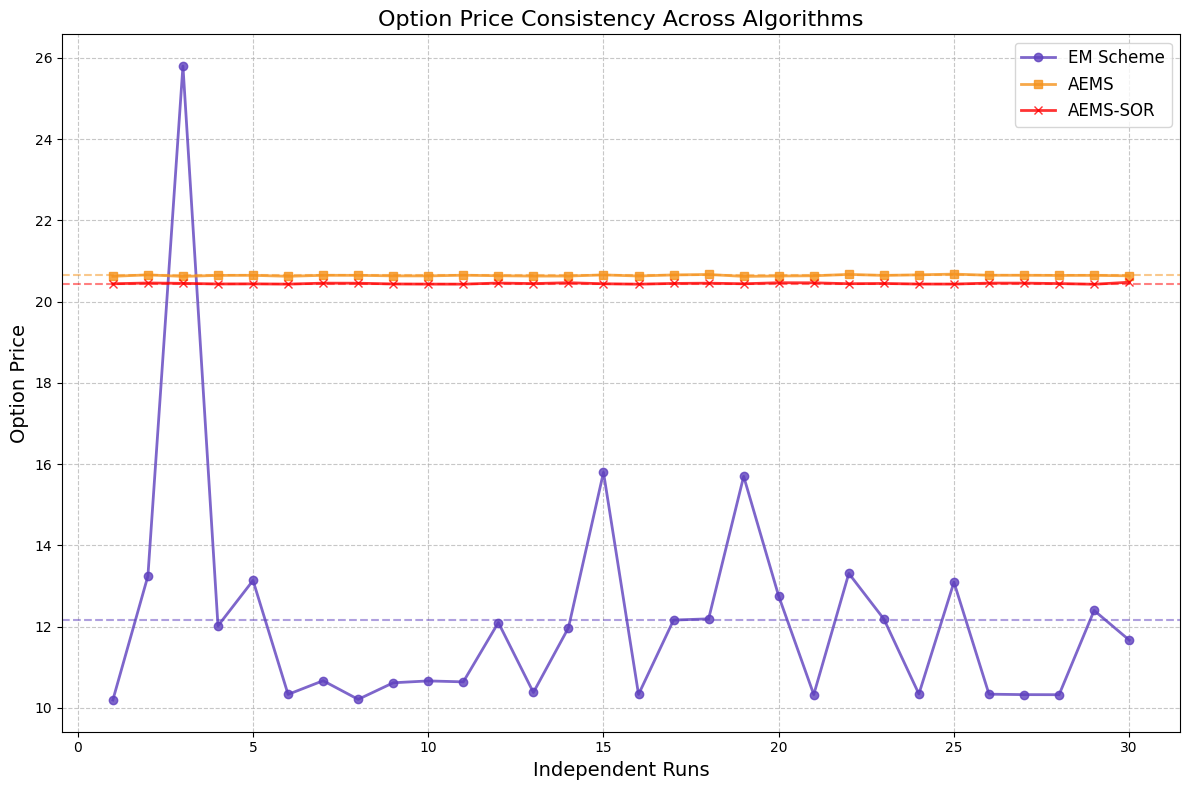
\includegraphics[width=\linewidth,height=0.72\textheight,keepaspectratio]{../Figures/PaperB/basket_option.png}
    \end{column}
    \begin{column}{0.34\textwidth}
      \begin{block}{Interpretation}
        The basket option experiment illustrates stability across repeated runs: EM fluctuates more, while AEMS and AEMS-SOR are visibly steadier.
      \end{block}
    \end{column}
  \end{columns}
\end{frame}

\begin{frame}{Paper B: Contribution and Limitations}
  \begin{columns}[T,onlytextwidth]
    \begin{column}{0.48\textwidth}
      \begin{block}{Contribution}
        \begin{itemize}
          \item Develops AEMS for Gatheral DMR by combining AES-type variance sampling with a Milstein correction.
          \item Introduces AEMS-SOR as a second-order refinement.
          \item Tests vanilla, barrier, forward volatility swap, and basket-style payoffs.
        \end{itemize}
      \end{block}
    \end{column}
    \begin{column}{0.48\textwidth}
      \begin{block}{Limitations}
        \begin{itemize}
          \item AEMS-SOR is not the most accurate scheme in every payoff and moneyness case.
          \item Most option benchmarks are numerical, not analytical.
          \item Improved path simulation does not remove the high-dimensional LSMC regression problem.
        \end{itemize}
      \end{block}
    \end{column}
  \end{columns}

  \vspace{0.45em}
  \begin{center}
    \small Paper C keeps the early-exercise setting and changes the numerical focus to continuation-value approximation.
  \end{center}
\end{frame}
